%%%%%%%%%%%%%%%%%%%%%%%%%%%%%%%%%%%%%%%%%%%%%%%%%%%%%%%%%%%%%%%%%%%%%%%%%%%%%%%%%%%%%%%%%%%%%%%%%%%%%%%%%%%%%%%%%%%%%%%%%%%%%%%%%%%%%%%%
% This is just a template to use when submitting manuscripts to Frontiers, it is not mandatory to use frontiers.cls nor frontiers.tex  %
%%%%%%%%%%%%%%%%%%%%%%%%%%%%%%%%%%%%%%%%%%%%%%%%%%%%%%%%%%%%%%%%%%%%%%%%%%%%%%%%%%%%%%%%%%%%%%%%%%%%%%%%%%%%%%%%%%%%%%%%%%%%%%%%%%%%%%%%

\documentclass{frontiersSCNS} % for Science articles
%\documentclass{frontiersMED} % for Medicine articles

\usepackage{url}

%\usepackage{lineno}
\usepackage{todonotes}
\usepackage{subfigure}
\usepackage{listings}
\lstset{language=python,
        basicstyle=\ttfamily,
        frame=single,xleftmargin=\fboxsep,xrightmargin=-\fboxsep}

% Absolute numerotation for figures
\usepackage{caption}
\captionsetup{figurewithin=none}  
\captionsetup{tablewithin=none}


\newcommand{\alex}[1]{\todo[inline, color=green!40]{#1}}
\newcommand{\fabian}[1]{\todo[inline, color=blue!40]{#1}}



%\linenumbers


\copyrightyear{}
\pubyear{}
%\onecolumn
%%% write here for which journal %%%
\def\journal{Neurosciences}
\def\DOI{}
\def\articleType{}
\def\citing{\color{darkgray}\cite}
\def\keyFont{\fontsize{6}{11}\helveticabold }
\def\firstAuthorLast{Alexandre Abraham {et~al}} %use et al only if is more than 1 author

% XXX Review the order of authors

\def\Authors{Alexandre Abraham\,$^{1,2,*}$, Philippe Gervais\,$^{1,2}$, Fabian
Pedregosa\,$^{1,2}$, Andreas Muller, Jean Kossaifi, Michael Eickenberg, Alexandre Gramfort, Bertrand
Thirion\,$^{1,2}$ and Ga\"el Varoquaux\,$^{1,2}$}
% Affiliations should be keyed to the author's name with superscript numbers and be listed as follows: Laboratory, Institute, Department, Organization, City, State abbreviation (USA, Canada, Australia), and Country (without detailed address information such as city zip codes or street names).
% If one of the authors has a change of address, list the new address below the correspondence details using a superscript symbol and use the same symbol to indicate the author in the author list.
\def\Address{
    $^{1}$Parietal Team, INRIA Saclay-\^{I}le-de-France, Saclay, France\\
    $^{2}$Neurospin, I\textsuperscript{2}BM, DSV, CEA, 91191 Gif-Sur-Yvette, France}

% The Corresponding Author should be marked with an asterisk
% Provide the exact contact address (this time including street name and city zip code) and email of the corresponding author
\def\corrAuthor{Alexandre Abraham}
\def\corrAddress{Parietal Team, INRIA Saclay-\^{I}le-de-France, Saclay, France}
\def\corrEmail{alexandre.abraham@inria.fr}

% \color{FrontiersBlue} Is the blue color, used in the Journal name, in the title, and the names of the sections


% Example of table from template

% \begin{table}[!t]
% \processtable{Resolution Requirements for the figures\label{Tab:01}}
% {\begin{tabular}{lllll}\toprule
% Image Type & Description & Format & Color Mode & Resolution\\\midrule
% Line Art & An image composed of lines and text,  & TIFF, EPS, JPEG & RGB, Bitmap & 900 - 1200 dpi\\
%            & which does not contain tonal or shaded areas.& & &\\
%            Halftone & A continuous tone photograph, which contains no text. & TIFF, EPS, JPEG & RGB, Grayscale & 300 dpi\\
% Combination & Image contains halftone + text or line art elements. & TIFF, EPS, JPEG & RGB,Grayscale & 600 - 900 dpi\\\botrule
% \end{tabular}}{This is a footnote}
% \end{table}


% Figures

% \textbf{Figure 1.}{ Enter the caption for your figure here.  Repeat as  necessary for each of your figures.}\label{fig:01}
% Don't add the figures in the LaTeX files, please upload them when submitting the article. Frontiers will add the figures at the end of the provisional pdf.


%%%%%%%%%%%%%%%%%%%%%%%%%%%%%%%%%%%%%%%%%%%%%%%%%%%%%%%%%%%%%%%%%%%%%%%%%%%%%%%
%%%%%%%%%%%%%%%%%%%%%%%%%%%%%%%%%%%%%%%%%%%%%%%%%%%%%%%%%%%%%%%%%%%%%%%%%%%%%%%
%%%%                                                                       %%%%
%%%%                          Naming convention                            %%%%
%%%%                                                                       %%%%
%%%%%%%%%%%%%%%%%%%%%%%%%%%%%%%%%%%%%%%%%%%%%%%%%%%%%%%%%%%%%%%%%%%%%%%%%%%%%%%
%%%%%%%%%%%%%%%%%%%%%%%%%%%%%%%%%%%%%%%%%%%%%%%%%%%%%%%%%%%%%%%%%%%%%%%%%%%%%%%

% Nifti world
% -----------
% - func_filename: name of a dataset file
% - func_img: name of a (loaded) nifti file
% - func_data, func_affine: data and affine of functional data

% Scikit-learn world
% ------------------
% - Xs: list of unmasked func_data (scikit-learn world)
% - X: unmasked func_data reduced to 2 dimensions (scikit-learn world)
% - y: labels

\begin{document}
\onecolumn
\firstpage{1}

\title[Machine Learning for Neuroimaging with Scikit-Learn]{Machine Learning for Neuroimaging with Scikit-Learn}
\author[\firstAuthorLast ]{\Authors}
\address{}
\correspondance{}
\editor{}
\topic{Research Topic}

\maketitle
\begin{abstract}

\section{}
Statistical learning methods are increasingly used to perform
neuroimaging analysis. Their main virtue for this type of application
is their ability to model high-dimensional datasets, e.g.\ multivariate
analysis of activation images, or capturing inter-subject variability.
Supervised learning is typically used in “decoding” setting to relate
brain images to behavioral or clinical observations, while
unsupervised learning is typically used to uncover hidden structure in
sets of images (e.g.\ resting state functional MRI) or to find
sub-populations in large cohorts of subjects. By considering
functional neuroimaging use cases, we illustrate how scikit-learn,
a Python machine learning library, can be used to perform some key
analysis steps. Scikit-learn contains a large set of statistical
learning algorithms, both supervised and unsupervised, that can be applied
to neuroimaging data after a proper preprocessing. Combined with other
Python libraries, neuroimaging data can be loaded, processed and the results
can be visualised easily.



\tiny
% XXX Fix keywords
%All article types: you may provide up to 8 keywords; at least 5 are mandatory.
\section{Keywords:} machine learning, statistical learning, neuroimaging, scikit-learn, python
\end{abstract}


\section{Introduction}

Python is being increasingly used in neuroimaging studies, \cite{millman2007analysis, hanke2009pymvpa}, which can be explained its
versatility, its ability to act as a glue between different components and the
maturity of its scientific stack.


\subsection{Scientific Python and neuroimaging ecosystem}

\subsubsection{Scipy and Numpy}

SciPy and NumPy packages are the basis of scientific computing in Python.
NumPy provides the \verb!ndarray! data type, an efficient $n$-dimensional data
representation. These vectors holds all common operations (transpose...) and
can be easily manipulated thanks to a simple, yet powerful, indexing scheme.
SciPy provides higher level mathematical functions that operate on ndarrays for
a variety of domains including linear algebra, optimization and signal
processing. Together, NumPy and SciPy provide a robust scientific environment
for numerical computing and they are the elementary bricks we use in all our
algorithms.

\subsubsection{Matplotlib}

Matplotlib is a Python plotting library that is tightly integrated into the
rest of the scientific python stack. It offers publication quality figures in
a variety of formats and allows to display plots, images or 3D plots in a
graphical user interface. All figures in this paper have been generated using
this library.


\subsubsection{Nibabel}

Nibabel is a neuroimaging data loading package. Nibabel can load or save data in
popular neuroimaging data format. This is indeed an entry point of all
our scripts.

\subsubsection{scikit-learn}

The {\em scikit-learn} project, \cite{pedregosa2011}, is an open source machine
learning library for the Python programming language. The ambition of the
project is to provide efficient and well-established machine learning tools within
a programming environment that is accessible to non-machine learning experts
and reusable in various scientific areas.


\section{Scikit-learn}

% Present the underlying concepts of scikit­learn: estimator,­ data
% representation, transformer...

All objects within scikit-learn share a uniform common basic API consisting of three
complementary interfaces: an \textit{estimator} interface for building and
fitting models, a \textit{predictor} interface for making predictions and a
\textit{transformer} interface for converting data into a different representation.

Interoperation with third-party code is made not on base on inheriting from a
particular class but on the base of implementing the appropriate methods for a
given interface.

\begin{itemize}
\item {\bf Estimator}. The \textit{estimator} interface is at the core of the library. It exposes a
    \texttt{fit} method for learning a model from training data.  All supervised
    and unsupervised learning algorithms (e.g., for classification, regression or
    clustering) are offered as objects implementing this interface. Machine
    learning tasks like feature extraction, feature selection or dimensionality
    reduction are also provided as estimators.

\item {\bf Predictor}. The \textit{predictor} interface extends the notion of an estimator
    by adding a \texttt{predict}
    method that takes an array \texttt{X\_test} and produces
    predictions for \texttt{X\_test}, based on the learned parameters of the
    estimator (we call the input to \texttt{predict} ``\texttt{X\_test}'' in order
    to emphasize that \texttt{predict} generalizes to new data). In the case of
    supervised learning estimators, this method typically returns the predicted
    labels or values computed by the model.

\item {\bf Transformer}. Since it is common to modify or filter data before feeding it to a learning
    algorithm, some estimators in the library implement a \textit{transformer}
    interface which defines a \texttt{transform} method. It takes as input some new
    data \texttt{X\_test} and yields as output a transformed version of
    \texttt{X\_test}. Preprocessing, feature selection and dimensionality reduction
    algorithms are all provided as transformers within the library. If the transformation
    can be inverted, a method called \verb!inverse_transform! also exists.

\end{itemize}

{\em scikit-learn} also offers a way to concatenate Estimators (known as
pipelining) and offers some routines for model selection.

\subsection{Model selection and cross validation}

The problem of model selection is to find, within some space, the best
combination of hyper-parameters with respect to some user-specifed criterion,
usually the prediction score on unseen data.

In {\em scikit-learn}, model selection is supported in two distinct
estimators, \texttt{GridSearchCV} and \texttt{RandomizedSearchCV}.  They take
as input an estimator (basic or composite), whose hyper-parameters must be
optimized, and a set of hyperparameter settings to search through. This set is
represented as a mapping of parameter names to a set of discrete choices in
the case of grid search, which exhaustively enumerates the ``grid'' (cartesian
product) of complete parameter combinations. Randomized search is a smarter
algorithm that avoids the combinatorial explosion in grid search by sampling a
fixed number of times from its parameter distributions.

\fabian{should we put an example here ?}

\section{From MR volumes to a data matrix}

At this point, we suppose that standard preprocessings have been applied to the
data (motion correction, slice timing, coregistration on a common template like
MNI if necessary).

\subsection{Transformation matrix}

Neuroimaging data are represented by 3D scans composed of voxels and their
associated timeseries along with a transformation matrix (called affine)
used to transpose the data in its original space.
Such matrix is needed because data may be anisotropic: the distance between
two voxels is not the same depending on the direction.
It is crucial to take that into account when dealing with
algorithms that uses the geometric structure of the data (see Searchlight
\ref{searchlight}).

One way to take it into account is to transform the coordinates. Going from
numpy indexing \verb!array[i, j, k]! to real coordinates $(x, y, z) \in
\mathbb{R}^3$ is a simple matrix product:

\[
    \begin{bmatrix}
        r_x & 0   & 0   & o_x \\
        0   & r_y & 0   & o_y \\
        0   & 0   & r_z & o_z \\
        0   & 0   & 0   & 1   \\
    \end{bmatrix}
    \begin{bmatrix}
        i \\
        j \\
        k \\
        1 \\
    \end{bmatrix}
    =
    \begin{bmatrix}
        x \\
        y \\
        z \\
        1 \\
    \end{bmatrix}
\]

We can write a Pyhton helper function to transpose coordinates of a mask into
its original space:

% I use that in the Searchlight example

% XXX: Gael: you are getting too much into the details, here
\begin{lstlisting}
def get_real_coordinates(mask, affine):
    # get coordinates of non zero voxels
    mask_coords = np.where(mask != 0)
    # add an extra dimension for the offset
    mask_coords = mask_coords + (np.ones(len(mask_coords[0]), dtype=np.int),)
    # apply the transformation
    mask_coords = np.dot(affine, np.asarray(mask_coords))[:3].T
    return mask_coords
\end{lstlisting}

This affine matrix can be different across files, e.g. when dealing when
multi-subject dataset or when using an external mask. In this case, it is very
important to resample all files on the same affine (see \ref{resampling}).

\subsection{Resampling}
\label{resampling}

Resampling consists in changing the spatial resolution of the data. This is
typically needed
when dealing when data coming from an heterogenous dataset, as shape depends
on acquisition parameters.

Resampling is an interpolation and may alter the data integrity. That is
why it should be used carefully. Oversampling (increasing
data resolution) leads to higher memory consumption and computation resources
with no gain in information.
Downsampling is commonly used to reduce the size of the data to process.
Typical sizes are 2mm or 3mm resolutions, but the spread of high field MR
scanner tends to lower these values.

For implementation, one should refer to \texttt{scipy.ndimage.affine\_transform}.

\subsection{Signal cleaning}

Now that 3D scans have been resampled, we have to take care of the time series
who stills have trends and scanner artifacts.

\subsubsection{Detrending} is an essential step when dealing with fMRI data. It removes a
linear trend over the time series of each
voxel. It is needed when you want to study the correlation between
features. You have to use \texttt{scipy.signal.detrend}.
\subsubsection{Normalization} is necessary for most processings.
\subsubsection{Confound removal} consists in regressing out confounds like
estimated movements. Some datasets provide csv files that can be used to remove
these artifacts.
\subsubsection{Signal filtering}. Low-pass filtering improves specificity.
High-pass filtering should be kept small, to keep some sensitivity.

\subsection{Masking}

\subsubsection{From 4-dimensional image to 2-dimensional array}

Neuroimaging data are represented in 4 dimensions: 3 dimensions for the scans,
which are positioned in a coordinate space, and one dimension for the time.
Scikit-learn algorithms, on the other hand, only accept 2-dimensional data: one
dimension for the features and one for the samples. This format brings \textit{i)}
consistency across all scikit-learn objects \textit{ii)} fast array iteration
\textit{iii)} compressed sparse representation thanks to NumPy.
In most
cases, voxels will be considered as features and timeseries as samples (these
roles are inversed for clustering methods because they group samples).\\


In order to use neuroimaging data in the scikit-learn, a
conversion is needed. The most simple way to achieve that would be to
\emph{flatten} the 3D scans into a 1D array. However, we know that not every
voxels in a neuroimaging scan is useful. In particular, outter-brain voxels are
of no use and, worse, they can bring spurious noise and scanner artefacts (such
as ghosts).\\

To sort out voxels of interest, we will apply a mask on the data (which is
already provided is most of public datasets).

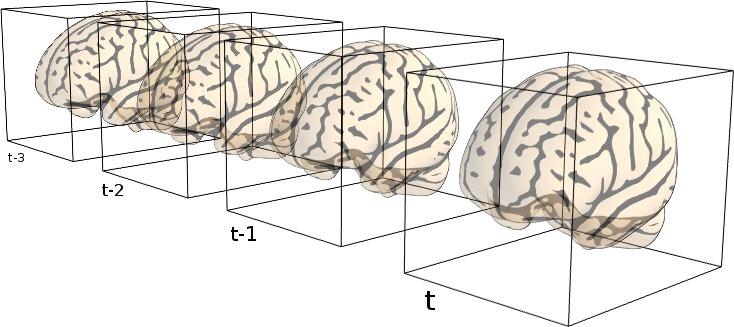
\includegraphics[width=.5\linewidth]{img/niimgs.jpg}

The implementation of masking procedure is fairly simple thanks to NumPy fancy
indexing. Special attention must be paid to the type of the mask array: it must
be boolean otherwise it will be considered as broadcasting and fill your memory.
2-dimensional masked data will be refered as \texttt{X} to follow scikit-learn
convetions.

\begin{lstlisting}
def apply_mask(mask_data, mask_affine, func_data, func_affine):
    assert(np.all(mask_affine == func_affine))
    mask_data = mask_data.astype(np.bool)
    X = func_data[mask_data].T
    return X

def unmask(X, mask_data, mask_affine):
    func_data = np.zeros(mask_data.shape, dtype=X.dtype)
    func_data[mask_data] = X
    return func_data, mask_affine

% For single subject data
X = apply_mask(mask_data, mask_affine, func_data, func_affine)
\end{lstlisting}


% This part has been removed because automatic masking is overly complicated and
% does not brinautomatic masking is overly complicated and does not bring much
% to the paper.

% \subsubsection{Automatically computing a mask}

% The simplest strategy to compute a mask is a binarization by a selected threshold.
% Due to the nature of the neuroimaging data, there exists some strategy to choose
% this threshold in order to obtain a decent segmentation.

% \alex{There is a reference for the method used in Nisl. We should put it there
% and in the code. Add a figure with an histogram to illustrate.}

% Multi subject computation is simply done by intersecting subjects maps
% relatively to a chosen threshold.

\subsubsection{Preserving geometrical structure}

Applying a mask on the data obviously remove the 3-dimensional structure of the
data. However, some algorithms, like the Ward, need this structural information.
\verb!sklearn.feature_extraction.image! provides two methods that builds an
adjacency matrix based upon your data while taking the mask into account:
\begin{itemize}
    \item \verb!grid_to_graph! creates a binary adjacency graph based upon the
        data shape. This is useful for Ward's clustering.
    \item \verb!image_to_graph! creates a distance matrix using the gradient of
        the image. This graph can be used in Spectral clustering.
\end{itemize}

\subsection{Label shifting}

Functional MRI measures brain activity by using the Blood-Oxygen-Level-Dependent
contrast (BOLD). In fact, like muscles, brain regions consume more oxygen and
nutriments when stimulated. So when a part of the brain starts working,
physiological mechanisms induce an oxygen-rich blood flood toward this
particular region: this is called haemodynamic response.

However, this reaction takes time, usually around 3-4 seconds. This is the
duration between the event and the reaction observed in the brain. To be able to
match these two events, we will sometimes have to shift our data. The number of
scans that must be shifted depends on the TR (repetition time) of the data.
Usually, we remove the first two scans of the data and the two last values of the
labels (to keep an homogeneous length).

\begin{lstlisting}
X = X[2:]
y = y[:-2]
\end{lstlisting}

\section{Decoding}

The process of predicting behavioral or phenotypic data from fMRI scan is
called decoding.

\subsection{SVM}

\subsubsection{Haxby dataset}

For this example and the following, we will use the Haxby dataset
(\cite{haxby2001}).
The Haxby dataset is from a study about face and object representation into the
brain (in particular in high-level visual cortex). It is composed of 12 runs for
each of the 6 subjects. Grayscale images representing faces, houses, cats,
bottles, scissors, shoes, chairs and random textures were presented in
24-second blocks separated by rest periods. The repetition time (TR) between each
scan is 2.5s. Full acquisition information are available in the reference paper.

To make this example easier, we will work on a subset of this dataset. We will
consider only one subject and will classify faces versus houses.

\subsubsection{Feature selection: ANOVA F-Test}

Even if the resolution of brain-imaging data seems low (3mm cubes, around 100000
neurones), from a computational point of view, this is huge. For example,
Haxby dataset has a resolution of $64\times64\times40 = 163840\text{ voxels}$.
After applying the mask, only 39912 voxels are left, which is still high.

In order to reduce the number of features, we can aggregate them (in regions of
interest for example) or we can select only the most relevant ones (those who
correlates most with the task). As we expect a lot of feature to be irrelevant
for our task, we opt for a feature selection method.

In supervised learning, the most popular feature selection method is the
ANalysis Of VAriance (ANOVA) F-Test. This is a generalization of the t-test to
more than 2 features. ANOVA compares several
groups to determine if they are similar (i.e. randomly drawn from the same
population, this is the null hypothesis). We use it to compare the distribution
of feature values across classes.

\verb!sklearn.feature_selection! contains a panel of feature selection
strategies. One can choose to take a percentile of the features
(\verb!SelectPercentile!), or a fixed number of features (\verb!SelectKBest!)
for example. All these objects are implemented as transformers.
Here we use a fixed number of features and we use the \verb!f_classif! function
(ANOVA F-Test) for scoring.

\begin{lstlisting}
from sklearn.feature_selection import SelectKBest, f_classif

### Define the dimension reduction to be used.
# Here we use a classical univariate feature selection based on F-test,
# namely Anova. We set the number of features to be selected to 500
feature_selection = SelectKBest(f_classif, k=500)
\end{lstlisting}

\subsubsection{Classification}

A Support Vector Classifier (SVC) is a simple classifier that finds a linear
hyperplane that separates the samples. Classifying a new sample boils down to
seeing on which side of the hyperplane the example is. SVC has the advantage to
give reliable results even when the number of dimensions is greater than the
number of samples.

The decision is taken based upon a subset of training data called support
vectors. We can say that these support vectors hold the information allowing to
discriminate the two classes, this is why we will display them and try to see if
they match some neuroscientific knowledge.

\begin{lstlisting}
from sklearn.svm import SVC
clf = SVC(kernel='linear', C=1.)
clf.fit(?)

### Look at the discriminating weights
svc = clf.support_vectors_
# reverse feature selection
svc = feature_selection.inverse_transform(svc)
\end{lstlisting}

\subsubsection{Pipeline}

The workflow described above (feature selection + estimator) is a standard one.
In fact, in most cases, the workflow will consist in atomic steps
\textit{linked} together (the output of a step is the input of the next one).
For this purpose, scikit-learn offers a pipeline object that allows such
linking. A pipeline is simply a list of scikit-learn objects through which the
input data will be conveyed. The function to call for each object (transform,
fit...) depends on its type.
This allow the developpers to write a complete processing as a one-liner.

\begin{lstlisting}
from sklearn.pipeline import Pipeline
anova_svc = Pipeline([('anova', feature_selection), ('svc', clf)])
\end{lstlisting}

\subsubsection{Results}

We display here the support vectors of the classifiers. These are the features
used by the classifier to discriminate between face and houses. Green and blue
lines surround features exhibited in the reference paper. We can see that our
classifier uses mostly voxels presents in the regions used to discriminate
houses.

\textbf{Figure \ref{fig:haxby}.}{Voxel importance in prediction decision for Haxby experiment
using \textit{a.} SVC, \textit{b.} Searchlight and \textit{c.} f\_score}{fig:01}

\subsection{Searchlight}
\label{searchlight}
For this example, we use the same dataset as the first one (one subject from
Haxby).

\subsubsection{Principle}

This Searchlight algorithm presented in \cite{kriegeskorte2006} aims to score
brain voxels depending on the amount of information they hold. The underlying
principle is the same as the previous example: each voxel in the brain is used
to predict the labels.

However, considering the fact that the information of a voxel is not only
contained in the voxel itself but in its neighbours, Kriegeskorte decided to run
a whole classification pipeline (learning and cross validation) in a ball
centered on the voxel, instead of applying a smoothing.

\subsubsection{Implementation}

Even if this algorithm seems complicated, it can be easily implemented thanks to
some basic bricks provided by the scikit learn. They key elements here are
\textit{i)} the neighbourhood (\verb!sklearn.neighobors.NearestNeighbors!),
\textit{ii)} the classifier (\verb!sklearn.svm.LinearSVC!),
\textit{iii)} the cross-validation (\verb!sklearn.svm.LinearSVC!).

As Searchlight is computationnaly expensive, we will add one constraint to our
code: it should be able to run on part of the mask. Thus we will have the
traditionnal \verb!mask! and a \verb!process_mask! that restraint computation
only to some voxels (in our case, a half axial slice).

First, we compute an adjacency graph between voxels. 
We build (fit) a connectivity graph on the mask using \texttt{NearestNeighbours}
but take the connectivity graph restrained to the
process mask so that the graph contains only our voxels of interest.

fitting a \verb!NearestNeighbours! on the \verb!mask! and applying it on
\verb!process_mask!.

\begin{lstlisting}
# Compute world coordinates of all in-mask voxels.
mask_coords = get_real_coordinates(mask_data, mask_affine)

# Compute world coordinates of all in-process mask voxels
process_mask_coords = get_real_coordinates(process_mask_data,
                                           process_mask_affine)

clf = neighbors.NearestNeighbors(radius=radius)
A = clf.fit(mask_coords).radius_neighbors_graph(process_mask_coords)
\end{lstlisting}

Then, for each row of our adjacency matrix, we do a cross validation using a
given estimator. This is the core of the algorithm and we see that it can be
written with a simple for-loop.

\begin{lstlisting}
scores = np.zeros(len(A.rows))
for i, row in enumerate(A.rows):
    scores[i] = np.mean(
            cross_val_score(estimator, X[:, row], y,
                            score_func=score_func,
                            cv=cv, n_jobs=1))
return scores
\end{lstlisting}

\subsubsection{Results}

Results are presented in figure \ref{fig:haxby}. Searchlight result is centered
and f\_score is on the right.
In order to evaluate the performance of Searchlight, we compare it to the
f\_score measure which is the simplest statistical test we can make on the data.
We can see that Searchlight localizes information mainly in the region of
interest corresponding to house. The smoothing effect is inherent to Searchlight
and is caused by the fact that a ball is used to iterate on the voxels.

\subsection{Classification of M/EEG sensor space data}

\alex{For the moment we don't have enough space and A. Gramfort told that this
may not fit as the whole paper is very fMRI oriented}

\subsection{Decoding: reconstructing image from brain activity}

\subsubsection{Kamitani dataset}

Kamitani dataset is based on a visual task like Haxby. In this experiment,
several series of $10\times10$ binary images are presented to two subjects.
Our goal will be to use the scikit-learn to learn a correlation between brain
activation and pixel color. Full details are available in the reference paper
(\cite{miyawaki2008}).

Kamitani training set is composed of random images (where black and white pixels
are balanced). The testing set is composed of structured images containing
geometric shapes (square, cross...) and letters.

There are two ways to establish a link between brain voxels and image pixels: we
can either try to reconstruct image from brain voxel activation, this is called
decoding, or we can try to predict brain activation from an image, this is called
encoding.

In the present example, we will do both encoding and decoding and see if the
results match.

\subsubsection{Principle} % Should be 'protocol'?

Common pre-treatment have been applied to the data (detrending and
standardization).

In the original paper (\cite{miyawaki2008}), Miyawaki uses a sparse multinomial
logistic regression and a sophisticated multiscale strategy to reconstruct the image.
For this use case, we will compare a l1 logistic regression and an Orthogonal
Matching Pursuit (\cite{mallat1993}). The OMP is a linear model that uses
timeseries as a dictionary and an l1 constraint on the loadings. Its
paritcularity is to add one atom at each step and update all coefficients
based on the orthogonal projection on preivously selected atoms.

To measure the performance of each approach, we will use a log of the
reconstruction error, which is closed to a log likelihood. Thanks to
scikit-learn, applying a cross validation to get score is a oneliner.

\begin{lstlisting}
from sklearn.linear_model import OrthogonalMatchingPursuit as OMP
from sklearn.cross_validation import cross_val_score

pipeline_OMP = Pipeline([('selection', SelectKBest(f_classif, 500)),
                         ('clf', OMP(n_nonzero_coefs=20)])
scores_omp = [cross_val_score(pipeline_OMP, X_train, y,
                              score_func=log_score, cv=5)
              for y in y_train]
\end{lstlisting}

\subsubsection{Results}

As Miyawaki, in figure \ref{fig:omp} we observe that reconstruction is more accurate in the fovea. This
may be caused by the fact that there are more neurons dedicated to foveal
representation in the primary visual area than for the borders.

\textbf{Figure \ref{fig:omp}.}{Reconstruction accuracy depending on pixel
position in the stimulus.}\label{fig:02}

\section{Encoding}

\alex{After talking with Michael, he told me that he could make a fairly simple
    example for encoding, which I think is a plus for the paper. The example will
    be integrated in Nisl.}

\section{Functional Connectivity}

In \cite{biswal1995}, Biswal was the first to exhibit coherent patterns in the
brain activation during resting state. These correlated voxel activations seemed
to form functional networks concording with neuroscientific knowledge.

Resting-state fMRI is useful when dealing with subjects that cannot execute a
specific task. In fact, no task-driven protocol is capable of diagnosing precisely
damaged brain areas in stroke patients, as no task can highlight these problems.
\cite{varoquaux2010b} exhibits differences in correlation between functional
networks between control and post-stroke patients.

As resting state fMRI are unlabeled data, we have to use unsupervised methods to
mine them. The most popular method to extract functional networks is ICA and
is the subject of our first use case. We will then show results obtained with
clustering methods as several efficient implementations are available in
scikit-learn.

The main problem with functional connectivity (and unsupervised methods in
general) is the lack of labels or ground truth. It is therefore very difficult
to score the computed models and cross validate it. At first, you can
compare your results with some reference atlas or neuroscientific knowledge. In
fact, it is believed that functional network should match anatomical division
\alex{Well, I believe that. Any reference ?}. It is also possible to relate to
networks discovered in task or other resting state experiments (eg default mode
network, visual and auditory networks...). Some researchers even released
functional atlases built upon one of their experiment (cite yeo, smith,
craddock).

\subsection{Independent Component Analysis (ICA)}

\subsubsection{Principle}

A typical example is the \emph{cocktail party problem} where ICA separates the
voices of people using signal from several mikes.

ICA is historically the reference method to extract networks from resting state
fMRI \cite{biswal1999}. It is a blind source separation method. Its principle is
to separate a
multivariate signal into several components by maximizing their non-gaussianity.
Several strategies have been used to syndicate ICA
results across several subjects. \cite{calhoun2001a} proposes a dimension
reduction (using PCA) followed by a concatenation of timeseries, which we use
this example.
\cite{varoquaux2010} use dimension reduction and canonical correlation analysis
to aggregate subject data.

\subsubsection{Preprocessing}

ICA requires whitened timeseries to run properly. Scikit-learn FastICA takes care
of this step. However, we still detrend them because
FastICA does not look for linear trends, only constant one.

\subsubsection{Application}

The code to apply ICA is very straitforward. Note the trnasposition of data
matrix to apply it on the right dimension.

\begin{lstlisting}
from sklearn.decomposition import FastICA
X = np.vstack(Xs)
ica = FastICA(n_components=n_components)
components_masked = ica.fit_transform(data_masked.T).T
\end{lstlisting}

After computation, normalization and thresholding of the map is necessary to
obtain brain networks.

\subsubsection{Results}

In addition of classical ICA shown above, we have computed results using the
others evoked methods (CanICA, MELODIC). We can see that with each method we can
extract the default mode network, more or less precisely.

\textbf{Figure \ref{fig:ica}.}{Extraction of default mode network using \textit{a} Group ICA
  \textit{b} CanICA}\label{fig:03}

\alex{MELODIC is missing}

\subsection{Clustering}

\subsubsection{Principle}

A clustering method aggregates similar features into groups. Scikit-learn
provides different clustering algorithms, each one holding its own properties:

\begin{itemize}
    \item{\bf Ward's clustering} uses a bottom-up hierarchical approach. Features are
        progressively aggregated into clusters until a whole tree is built. This
        tree is then cut to get the requested number of clusters.
    \item{\bf k-means} is a centroid based approach. Clusters are represented by
        a central vector: a feature belongs to the cluster of the nearest
        centroid.
    \item{\bf spectral clustering} is a graph based approach. It separates
        the feature graph into subgraphs by maximizing intra-group connectivity and
        minimizing inter-group connectivity.
\end{itemize}

For each algorithm, one must specify the number of clusters. This parameter is
not easy to set as we have few information about the data.

In this use case, we will use Ward's clustering and will compare its results to
k-means and spectral clustering. Ward's clustering is fast and builds a complete
tree of features, such that varying the number of clusters is costless.

We use a PCA to reduce the dimensionality of the problem. We also apply
smoothing to k-means.

\begin{lstlisting}
connectivity = grid_to_graph(n_x=mask.shape[0], n_y=mask.shape[1],
                             n_z=mask.shape[2], mask=mask)
ward = WardAgglomeration(n_clusters=1000, connectivity=connectivity)
ward.fit(X)
\end{lstlisting}

\subsubsection{Results}

\textbf{Figure \ref{fig:clustering}.}{Brain decomposition using different clustering techniques.}\label{fig:04}


\section*{Disclosure/Conflict-of-Interest Statement}
%All relationships financial, commercial or otherwise that might be perceived
%by the academic community as representing a potential conflict of interest
%must be described. If no such relationship exists, authors will be asked to
%declare that the research was conducted in the absence of any commercial or
%financial relationships that could be construed as a potential conflict of
%interest.
The authors declare that the research was conducted in the absence of any
commercial or financial relationships that could be construed as a potential
conflict of interest.

\paragraph{Funding\textcolon} Text Text Text Text Text Text  Text Text.

\bibliographystyle{frontiersinSCNS} % for Science articles
\bibliography{biblio}

\newpage

\begin{figure}[h]
  \begin{center}
  \subfigure[SVC]{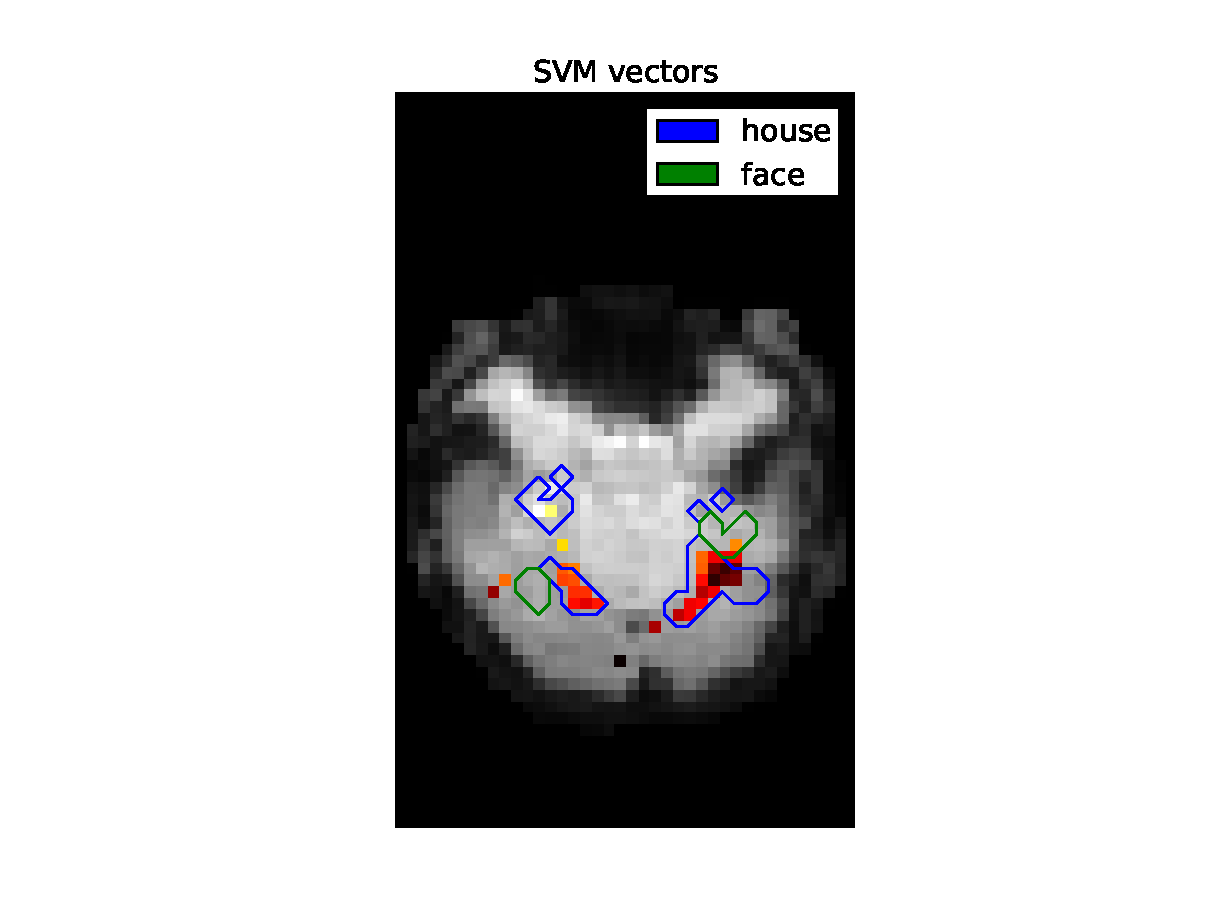
\includegraphics[width=.3\linewidth]{img/svm.pdf}}
  \subfigure[Searchlight]{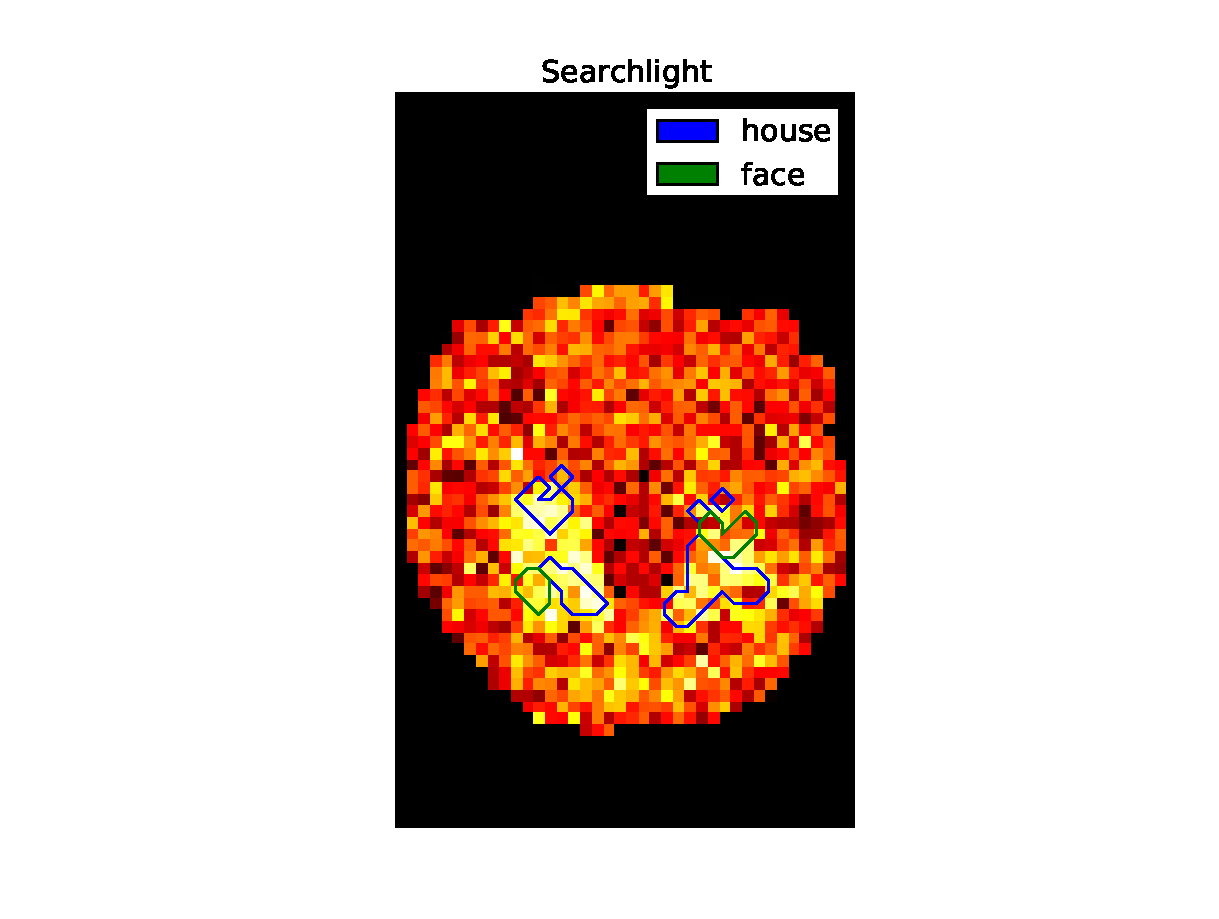
\includegraphics[width=.3\linewidth]{img/searchlight.pdf}}
  \subfigure[F\_score]{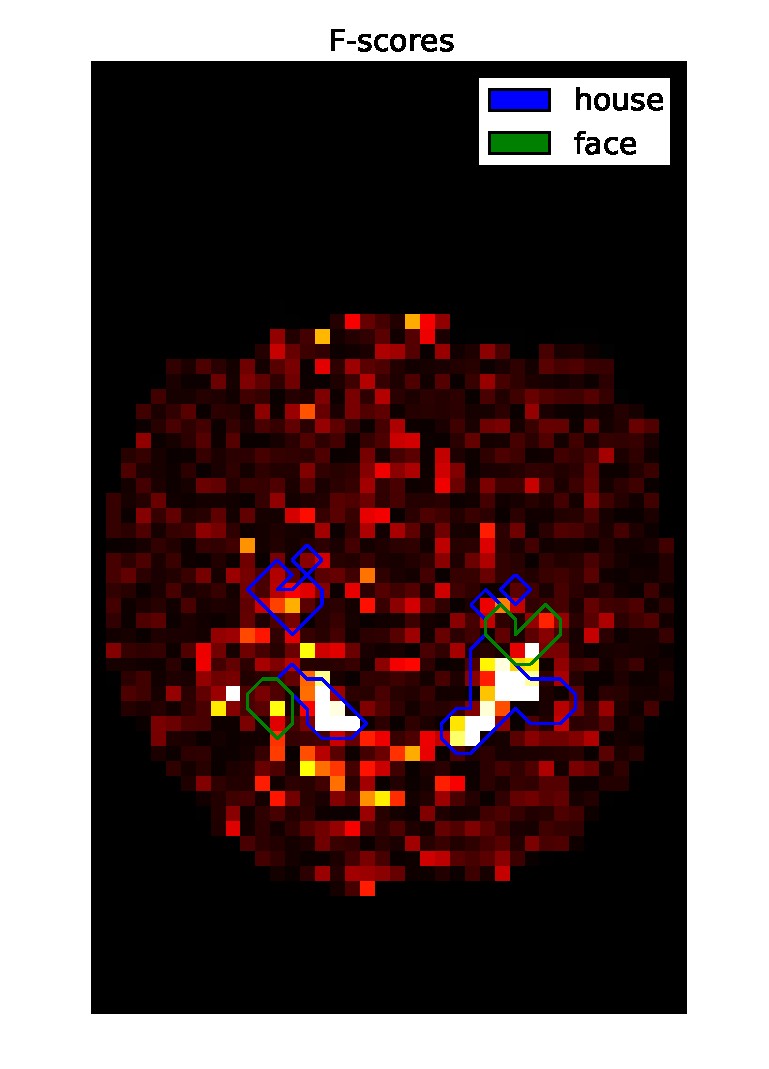
\includegraphics[width=.3\linewidth]{img/f_score.pdf}}
  \end{center}
\caption{Voxel importance in prediction decision for Haxby experiment
using \textit{a.} SVC, \textit{b.} Searchlight and \textit{c.}
f\_score}
\label{fig:haxby}
\end{figure}
\begin{figure}[h]
  \begin{center}
    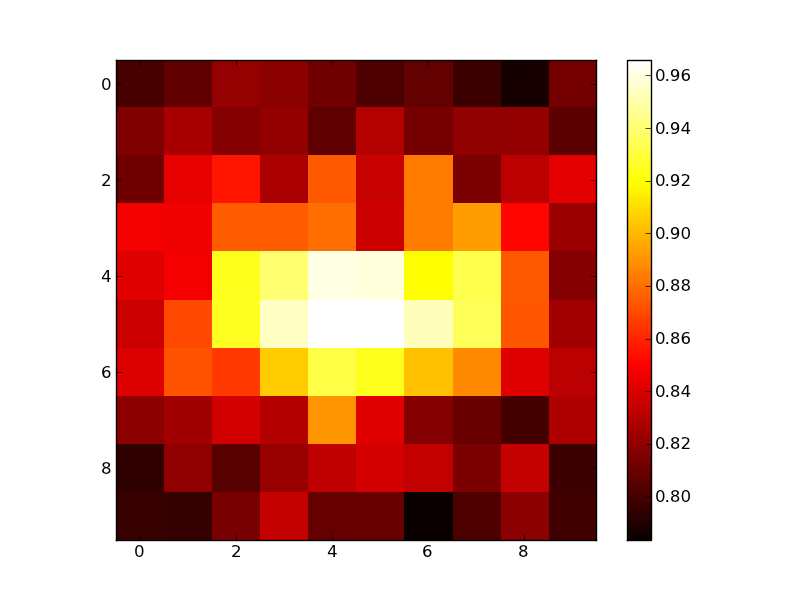
\includegraphics[width=.3\linewidth]{img/logistic_l1_scores.png}
  \end{center}
  \caption{Reconstruction accuracy depending on pixel
           position in the stimulus.}
\label{fig:omp}
\end{figure}

\begin{figure}[h]
  \begin{center}
      \subfigure[ICA]{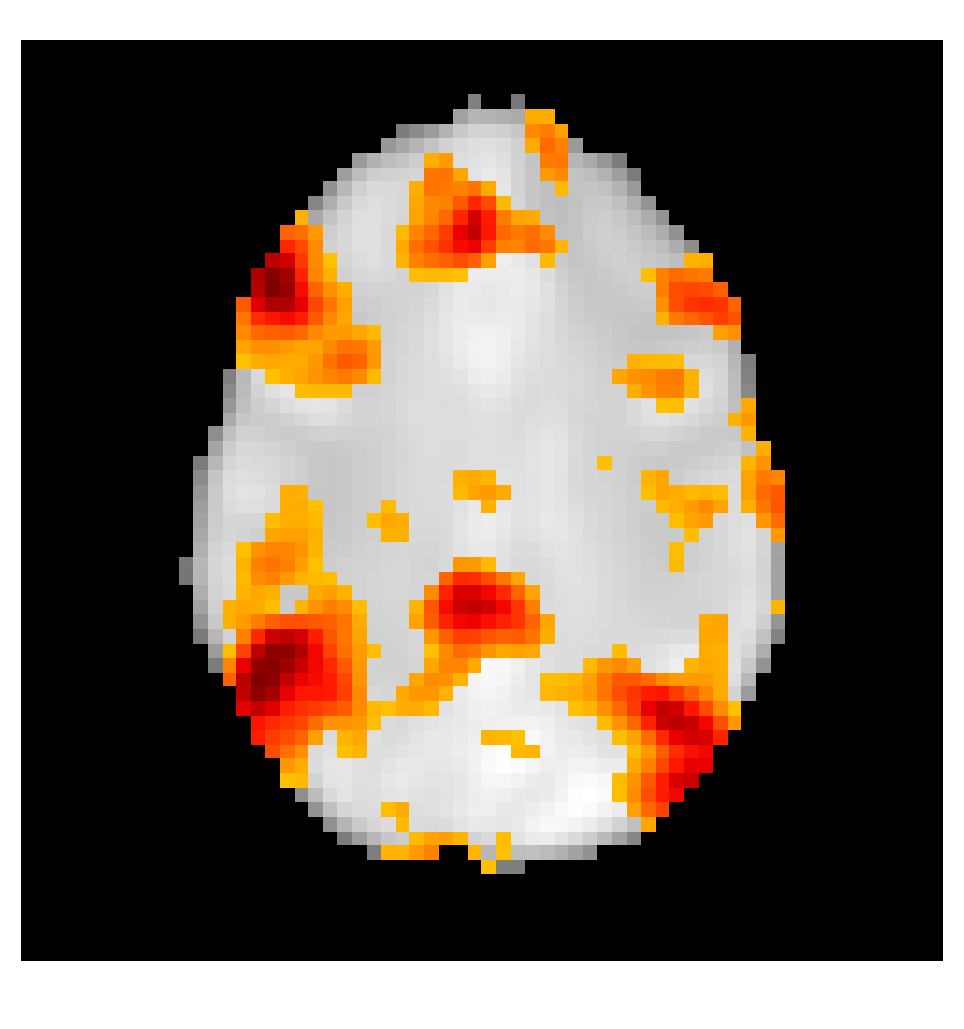
\includegraphics[width=.3\linewidth]{img/ica.pdf}}
      \subfigure[CanICA]{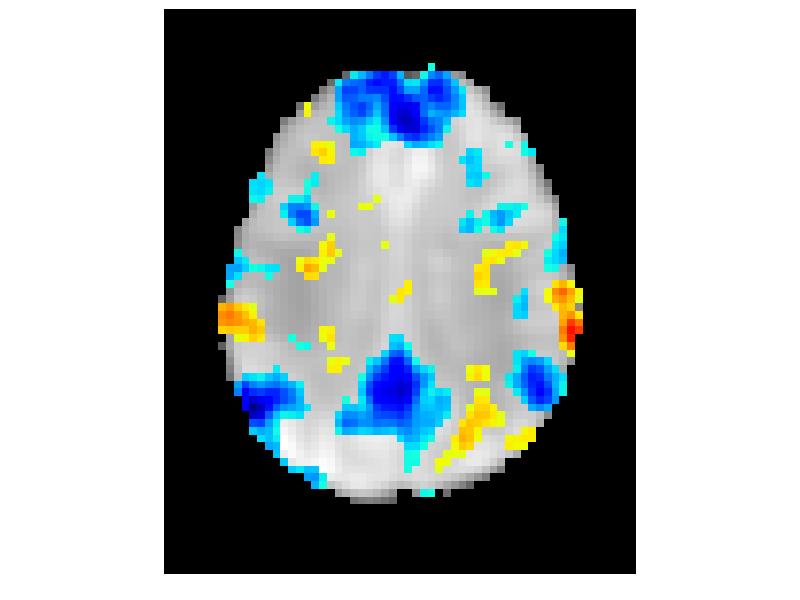
\includegraphics[width=.3\linewidth]{img/plot_canica_resting_state_17.png}}
  \end{center}
  \caption{Extraction of default mode network using \textit{a} Group ICA
  \textit{b} CanICA}
  \label{fig:ica}
\end{figure}

\begin{figure}[h]
  \begin{center}
  \subfigure[Ward's clustering]{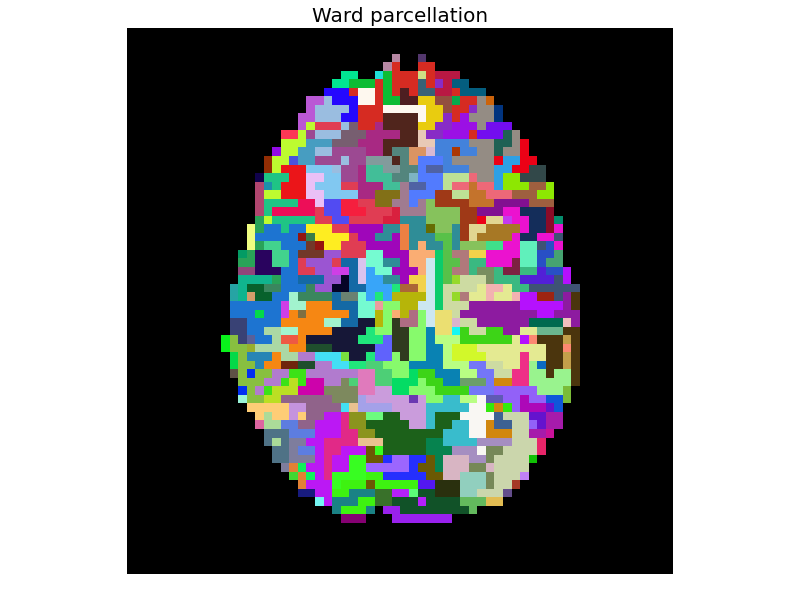
\includegraphics[width=.3\linewidth]{img/plot_rest_clustering_1.png}}
  \end{center}
  \caption{Brain decomposition using different clustering techniques.}
  \label{fig:clustering}
\end{figure}
\end{document}
